\documentclass{article}
\usepackage[utf8]{ inputenc }
\usepackage{ enumitem }
\usepackage{ bbm }
\usepackage{ mathtools }
\usepackage{ geometry}
\geometry{legalpaper, margin=1.3in}
\usepackage{ graphicx }
\graphicspath{ {img/} }
\usepackage{ algorithm }
% \usepackage{ algorithmic }
\usepackage[noend]{ algpseudocode }
\usepackage[toc,page]{appendix}
\usepackage{ tikz }
\usetikzlibrary{automata,positioning}
\usepackage{ hyperref }
\pdfinfo{
   /Author (Hugo Thomas & Hakim Amraoui)
   /Title  (MOGPL Project report, Sorbonne Université)
   /CreationDate (D:20211021195600)
}
\begin{document}

\begin{titlepage}
\begin{center}

\textsc{\LARGE Sorbonne Universite} \\[1cm]
\textsc{\LARGE Master 1 - Informatique} \\[1cm]
\textsc{\Large Année 2021/2022} \\[7cm]


{\huge \bfseries Rapport de projet} \\[0.5cm]
{\huge \bfseries -} \\[0.5cm]
{\huge \bfseries Modélisation, Optimitation, Graphes, Programmation linéaire}
\\[4cm]
{\LARGE Hugo THOMAS} \\[0.5cm]
{\LARGE Hakim AMRAOUI} \\[0.5cm]
\vfill
\includegraphics[scale=0.6]{su.png}
\end{center}
\end{titlepage}

\tableofcontents
\newpage


\section{Assertions sur les graphes}


\paragraph{Assertion 1 : } Un sous-chemin préfixe d'un chemin d'arrivée au plus
tôt peut ne pas être un chemin d'arrivée au plus tôt. \\
Soient $x, y$ deux sommets de $G$ et $P$ un chemin d'arrivée au plus tôt entre
$x$ et $y$. Montrons qu'il existe un sommet $y'$ tel qu'un sous-chemin préfixe
de $P$ n'est pas un chemin d'arrivée au plus tôt entre $x$ et $y'$. Considérons
le chemin d'arrivé le plus tôt entre $a$ et $l$, le chemin d'arrivée au plus tôt
est $a \rightarrow c \rightarrow h \rightarrow i \rightarrow l$, d'arrivé au
temps 8. Avec $y' = i$, on a un nouveau chemin d'arrivé qui est $a \rightarrow
f \rightarrow i$ au temps 5. L'assertion 1 est donc vérifiée.

\begin{figure}[h]
    \centering
    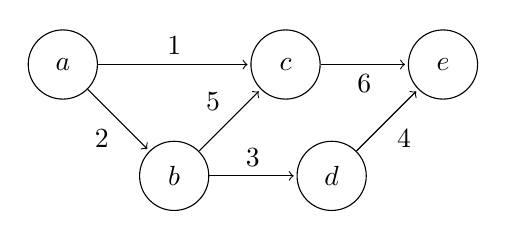
\begin{tikzpicture}[shorten >=1pt,node distance=2cm,on grid,auto]
        \node[state] (1)   {$a$};
        \node[state] (2) [below right=of 1] {$b$};
        \node[state] (3) [above right=of 2] {$c$};
        \node[state] (4) [right=of 2] {$d$};
        \node[state] (5) [right=of 3] {$e$};
        \path[->]
            (1) edge node {1} (3)
                edge node [swap] {2} (2)
            (2) edge node {5} (3)
                edge node {3} (4)
            (3) edge node [swap] {6} (5)
            (4) edge node [swap] {4} (5)
            ;
    \end{tikzpicture}
    \caption{Graphe G utilisé pour notre exemple de l'assertion 2}
\end{figure}

\paragraph{Assertion 2 : } Un sous-chemin postfixe d'un chemin de départ au plus
tard peut ne pas être un chemin de départ au plus tard. \\
Soient $x, y$ deux sommets de $G$ et $P$ un chemin de départ au plus tard entre
$x$ et $y$. Montrons qu'il existe sommet $x'$ tel qu'un sous-chemin postfixe de
$P$ entre $x'$ et $y$ n'est pas un chemin de départ au plus tard. En utilisant
le graphe $G$ de la figure 1, un chemin de départ au plus tard en allant de $a$ à
$e$ serait $a \rightarrow b \rightarrow d \rightarrow e$, de départ au temps 2.
Or, en prenant le sous-chemin postfixe de départ en $b$, le chemin obtenu $b
\rightarrow d \rightarrow e $ de départ au temps 3 n'est plus le chemin de
départ au plus tard. En effet, en partant de $b$, le chemin de départ au plus
tard serait $b \rightarrow c \rightarrow e$ de départ au temps 5. L'assertion 2
est donc vérifiée.

\paragraph{Assertion 3 : } Un sous-chemin d'un chemin le plus rapide peut ne pas
être un chemin le plus rapide. \\
Supposons qu'un sous-chemin d'un chemin le plus rapide est toujours un chemin le
plus rapide, et trouvons un contre-exemple dans le graphe $G$ du sujet. Entre
les sommets $a$ et $l$, un des chemins le plus rapide est le chemin $a
\rightarrow c \rightarrow h \rightarrow i \rightarrow l$ de durée 5. Considérons
le sous-chemin $a \rightarrow f \rightarrow i$, ce chemin de durée $3$ n'est pas
le chemin le plus rapide entre les sommets $a$ et $i$, en effet le chemin $a
\rightarrow i$ de durée 1 est plus rapide.
\paragraph{Assertion 4 : } Un sous-chemin d'un plus court chemin peut ne pas
être un plus court chemin. \\
Supposons qu'un sous-chemin d'un chemin le plus court est toujours un chemin le
plus court, et trouvons un contre-exemple dans le graphe $G$ du sujet.
Considérons de nouveau sommets $a$ et $l$, un des plus courts chemins est le
chemin $a \rightarrow f \rightarrow i \rightarrow l$. Considérons le sous-chemin
$a \rightarrow f \rightarrow i$, ce chemin de longueur $2$ n'est pas le chemin
le plus court entre les sommets $a$ et $i$, en effet le chemin $a \rightarrow i$
de poids 1 est plus court.


\section{Algorithmes pour les calculs des 4 types de chemins minimaux}
On suppose que l'on a accès à une implémentation de l'algorithme de Dijkstra,
sans en donner le pseudo code (il est dans le cours), par la procédure
\texttt{Dijkstra($d,f,G$)}, telle que \\
\begin{equation}
    \texttt{Dijkstra($d$,$f$,G)} = \begin{cases}
    \texttt{nil} & \text{s'il n'y a pas de chemin entre $d$ et $f$ dans $G$} \\
    \big(\mathcal{W}, \Pi\big) &\text{tels que }
    \mathcal{W}[i]\text{ est le poids du PCC jusqu'à $i$, et } \\
    & \Pi[i] \text{ est le prédécesseur de $i$ dans ce PCC}\\
\end{cases}
\end{equation}
La complexité temporelle de cette procédure est en $O\big((|V|+|E|)\log|V|\big)$ où $|E|$ est
le nombre d'arcs et $|V|$ est le nombre de sommets, via l'utilisation d'une file
de priorité. \\\noindent
Et d'autre part accès aux procédures suivantes :

\begin{itemize}[label=-]
    \item \texttt{bfs($G, s$)} : \textit{Graphe $\times$ Sommet $\rightarrow$ Tableau[Sommet]} :
    parcourt le graphe $G$ en largeur à partir de $s$ et retourne le tableau des prédécesseurs.
    La complexité temporelle de \texttt{bfs} est $O\big(|E|+|V|)$.
    \item \texttt{transpose($G$)}: \textit{Graphe $\rightarrow$ Graphe} :
    renvoie le graphe transposé de $G$.
    \item \texttt{renverse($l$)}: \textit{Liste $\rightarrow$ Liste} : renvoie la
    liste $l$ dont les éléments dans l'orde inverse
    \item \texttt{duree($P$)}: \textit{Chemin $\rightarrow$ Nombre} : renvoie la
    durée du chemin $P$
    \item \texttt{delimiter($\tilde{G},d, f, t_\alpha, t_\omega$)}:
    \textit{Graphe $\rightarrow$ Graphe} : renvoie $\tilde{G}$ tel qu'un chemin
    $s \rightarrow f$ $P$ dans $\tilde{G}$ respecte les contraintes $debut(P) >
    t_\alpha$ et $fin(P)<t_\omega$. Son pseudo code ne concernant pas
    directement les algorithmes de plus courts chemins, celui-ci est situé en
    annexe \ref{p-c-delimiter}.
\end{itemize}

Nous ne prenons pas en compte la compléxité de la transformation du graphe $G$
au graphe $\tilde{G}$, qui sera examinée juste en suivant. $|V|$ et $|E|$ sont donc
respectivement le nombre de sommets et le nombre d'arcs de $\tilde{G}$.

\subsection*{I. Arrivée au plus tôt}
\begin{algorithm}[h]
    \caption{Arrivée au plus tôt}
    \begin{algorithmic}[1]
    \Procedure{APT}{$d, f, \tilde{G}, t_\alpha, t_\omega$}
    \Comment{
        $d$ : Sommet de départ, $f$: Sommet de fin, $\tilde{G}$: le graphe}
    \State $PCC \leftarrow $ \texttt{nil} \Comment{PCC avec la contrainte APT}
    \State $T \leftarrow \infty$ \Comment{Jour d'arrivée au plus tôt}
    \State $\tilde{G} \leftarrow \texttt{delimiter($\tilde{G}, d, f, t_\alpha, t_\omega$)}$
    \State $G_T \leftarrow \texttt{transpose($\tilde{G}$)}$
    \ForAll{$u \in \tilde{V}_{in}(f)$}
        \State $pcc \leftarrow$ \texttt{bfs($G_T, s$)}
        \If{$tmp \neq \texttt{nil} \textbf{ and } t < T$}
            \State $T \leftarrow t$
            \State $PCC \leftarrow pcc$
        \EndIf
    \EndFor
    \State \Return $\texttt{renverse($PCC$)}$
    \EndProcedure
    \end{algorithmic}
\end{algorithm}
\paragraph{Idée de l'algorithme : } Il est très similaire à l'algorithme II.
On considère le graphe $G_T$ transposé de $G$, ainsi nous pouvons, à partir de
$f$, trouver un plus court chemin de $f$ à $d$ avec l'algorithme de Dijkstra. En
itérant sur tous les sommets de $\tilde{V}_{in}(f)$ et en conservant le chemin
dont le sommet de départ à la fois admet un chemin jusqu'à $s$ et dont le temps
de départ est minimal (dans $G_T$) l'algorithme renvoie le chemin d'arrivée au plus
tôt. Si dans $G_T$ il y a un chemin de $f$ à $d$, alors il y a un chemin de $d$
à $f$ dans $G$. Et un chemin de départ au plus tôt dans $G_T$ est un chemin
d'arrivée au plus tôt dans $G$.
% TODO : peut-être prouver un peu plus formellement les deux dernières phrases.
\paragraph{Complexité : } Si le graphe est représenté via une liste d'adjacence,
calculer son graphe transposé prend un temps en $O(|E|+|V|)$. L'appel à la
procédure \texttt{delimiter} prend aussi un temps en $O(|E|+|V|)$ (simple
parcours de tous les arcs de tous les noeuds). Il y a $d^+(f)$ éléments dans
$\tilde{V}_{in}(f)$ donc $d^+(f)$ appels à \texttt{bfs}, et $d^+(f) <<
|E|$. D'où une compléxité totale en
$O\big(|E|+|V|)$ si on suppose que $d^+(f)$ est constant devant $|E|$.


\subsection*{II. Départ au plus tard}
\begin{algorithm}[h]
\caption{Départ au plus tard}
\begin{algorithmic}[1]
    \Procedure{DPT}{$d, f, \tilde{G}, t_\alpha, t_\omega$}
    \Comment{
        $d$ : Sommet de départ, $f$: Sommet de fin, $\tilde{G}$: le graphe}
    \State $PCC \leftarrow $ \texttt{nil} \Comment{PCC avec la contrainte DPT}
    \State $T \leftarrow -\infty$ \Comment{Jour de départ au plus tard}
    \State $\tilde{G} \leftarrow \texttt{delimiter($\tilde{G}, d, f, t_\alpha, t_\omega$)}$
    \ForAll{$u \in \tilde{V}_{out}(d)$}
        \State $pcc \leftarrow$ \texttt{bfs($\tilde{G}, u$)}
        \If{$tmp \neq \texttt{nil} \textbf{ and } t > T$}
            \State $T \leftarrow t$
            \State $PCC \leftarrow pcc$
        \EndIf
    \EndFor
    \State \Return $PCC$
    \EndProcedure
    \end{algorithmic}
\end{algorithm}

\paragraph{Idée de l'algorithme : } Dans $\tilde{G}$ obtenu suite à la
transformation, on parcourt tous les états représentant le sommet de départ i.e.
$\tilde{V}_{out}(d)$, dans l'exemple 1, pour un départ depuis $a$, les sommets
(a,1), (a,2), (a,4). Pour chacun de ces sommets on applique l'algorithme de
Dijkstra afin de trouver le plus court chemin jusqu'à l'objectif. Un plus court
chemin obtenu de cette manière et conservé si et seulement s'il n'est pas nul et
son temps de départ $t$ est supérieur au plus grand temps de départ déjà
enregistré permettant d'arriver à l'objectif $T$.

\paragraph{Complexité : } Il y a $d^-(d)$ éléments dans $\tilde{V}_{out}(d)$, il
y a donc $d^-(d)$ appels à la procédure \texttt{bfs}, et $d^-(d) << |E|$. L'appel à la
procédure \texttt{delimiter} prend un temps en $O(|E|+|V|)$, et \texttt{bfs} est
également en $O(|E|+|V|)$. Donc une compléxité en
$O\big(|V|+|E|\big)$ si l'on suppose $d^-(d)$ toujours très petit.

\subsection*{III. Chemin le plus rapide}
\begin{algorithm}
\caption{Chemin le plus rapide}
\begin{algorithmic}[1]
\Procedure{CPR}{$d, f, \tilde{G}, t_\alpha, t_\omega$}
\Comment{
    $d$ : Sommet de départ, $f$: Sommet de fin, $\tilde{G}$: le graphe}
    \State $pcc \leftarrow \texttt{nil}$ \Comment{PCC avec la contrainte CPR}
    \State $D \leftarrow \infty$ \Comment{Durée du tel PCC}
    \State $\tilde{G} \leftarrow \texttt{delimiter($\tilde{G}, d, f, t_\alpha, t_\omega$)}$
    \ForAll{$u \in \tilde{V}_{out}(d)$}
        \State $tmp, p = \texttt{Dijkstra($u,f,\tilde{G}$)}$
        \State $d \leftarrow \texttt{duree($tmp$)}$
        \If{$pcc \neq \texttt{nil} \textbf{ and } d < D$}
            \State $D \leftarrow d$
            \State $pcc \leftarrow tmp$
        \EndIf
    \EndFor
    \State \Return $(pcc, D)$
\EndProcedure
\end{algorithmic}
\end{algorithm}
\paragraph{Idée de l'algorithme : } Encore une fois, en itérant sur tous les
sommets de $\tilde{V}_{out}(d)$ et en calculant la $duree(pcc)$ à partir de ce
sommet, on obtient la solution optimale en conservant le chemin qui minimise la
durée. La boucle sur tout les sommets sert à s'assurer que l'on essaye bien tous
les arcs sortants du sommet de départ. En effet, il n'est pas dit que la
solution optimale soit donnée dès la première itération, si celle-ci ne renvoie
pas un chemin passant par le sommet de départ du chemin optimal, aucun
traîtement sur le chemin obtenu ne permet d'obtenir la solution optimale.


\paragraph{Complexité : } Il y a $d^-(d)$ éléments dans $\tilde{V}_{out}(d)$, il y a donc
$d^-(d)$ appels à la procédure \texttt{Dijkstra}. Le calcul de la durée peut se faire en $O(1)$
Donc une compléxité en $O\big(d^-(d)(|V|+|E|)\log|V|\big)$.


\subsection*{IV. Plus court chemin}
\begin{algorithm}
\caption{Plus court chemin}
\begin{algorithmic}[1]
    \Procedure{PCC}{$d, f, \tilde{G}, t_\alpha, t_\omega$}
        \State $\tilde{G} \leftarrow \texttt{delimiter($\tilde{G}, d, f, t_\alpha, t_\omega$)}$
        \State \Return \texttt{Dijkstra($d,f,\tilde{G}$)}
    \EndProcedure
\end{algorithmic}
\end{algorithm}

\paragraph{Idée de l'algorithme : } Les graphes sont garantis sans circuit et
dans $\tilde{G}$ les arcs sont étiquetés par des poids $\lambda$ représentant la
distance entre deux sommets, les poids sont donc positifs ou nuls, l'utilisation
de l'algorithme de Dijkstra sur $\tilde{G}$ retourne donc le plus court chemin
entre $d$ et $f$ en terme de distance de manière efficace.

\paragraph{Compléxité : } Un seul appel à \texttt{Dijkstra} : compléxité en $O((|V|+|E|)\log|V|)$.

\section{Modélisation du problème PCC en programmation linéaire}
La résolution du problème de plus court chemin avec l'algorithme du simplexe
étant un problème usuel de programmation linéaire, nous n'avons rien inventé, et
nous sommes inspirés du cours de M. Artigues\cite{CA-DC}. Nous en
détaillerons tout de même le fonctionnement.

Considérons le graphe suivant, dans
lequel nous cherchons le plus court chemin entre les sommets $d$ et $f$.

Un plus court chemin de type IV minimise la distance $\lambda$ entre deux sommets, nous ne
nous intéressons donc pas aux temps $t$ de départ.

On introduit les variables $x_{ij}$ avec $i,j \in V $ qui vaut 1 si
l'arc $i\rightarrow j$ est dans le plus court chemin, 0 sinon.
Comme on recherche le plus court chemin, la fonction objectif à minimiser est
\begin{equation}
    \label{fun-obj}
    z = \sum_{i,j}\lambda_{ij}x_{ij}
\end{equation}
où $\lambda_{ij}$ est le poids de l'arc $i \rightarrow j$.

Il y a ensuite trois groupes de contraintes. Pour cela, on considère un
\textit{module} qui se déplacerait de sommets en sommets, et on rend compte de
sa position en se mettant à la place des sommets.
\\
\\
Premier groupe contraintes : le nombre d'arcs dans le chemin entrant en $d$ est
plus petit (de 1) que le nombre
d'arcs sortant de $d$.
\begin{equation}
    \label{cont-1}
    \sum_{k\in S^+(d)}x_{dk} - \sum_{k\in S^-(d)}x_{kd} = 1
\end{equation}
Ainsi on est sûr que le \textit{module} s'échappe du sommet $d$.
\\
\\
Deuxième groupe de contraintes : dans le chemin optimal, le nombre d'arcs entrants
et sortants d'un sommet qui n'est ni le départ ni la fin doivent être égaux
\begin{equation}
    \label{cont-2}
    \forall i \in V \backslash \{d, f\}: \sum_{k\in S^+(i)}x_{ik} - \sum_{k\in S^-(i)}x_{ki} = 0
\end{equation}
Ainsi le \textit{module} ne reste pas dans un sommet, sans s'occuper des cas $d$ et $f$.
\\
\\
Troisième groupe de contraintes : dans le chemin optimal le nombre d'arcs
entrants dans le sommet $f$ de fin est plus grand (de 1) que le nombre d'arcs
sortant de ce sommet.
\begin{equation}
    \label{cont-3}
    \sum_{k\in S^-(f)}x_{kf} - \sum_{k\in S^+(f)}x_{fk} = 1
\end{equation}
Ainsi, à la fin, le \textit{module} est dans le sommet $f$. Finalement, en
rassemblant la fonction objectif (\ref{fun-obj}) et les contraintes décrites en
(\ref{cont-1}), (\ref{cont-2}), et (\ref{cont-3}), nous obtenons le PL suivant
\begin{equation}
    \label{pl-P}
    (P)\begin{cases}
        \texttt{min } z = \sum_{i,j}\lambda_{ij}x_{ij} \\ \\

        \sum_{k\in S^+(d)}x_{sk} - \sum_{k\in S^-(d)}x_{ks} = 1\\
        \sum_{k\in S^+(i)}x_{ik} - \sum_{k\in S^-(i)}x_{ki} = 0, \forall i \in V \backslash \{d, f\}\\
        \sum_{k\in S^-(f)}x_{kf} - \sum_{k\in S^+(f)}x_{fk} = 1 \\ \\

        x_{ij} \in \{0, 1\}, \forall i, j \in V
    \end{cases}
\end{equation}


\subsection{Implémentation}
Le fichier \texttt{lp.py} contient l'implementation du programme linéaire
permettant de résoudre le problème de plus court chemin. Pour l'illustration,
nous cherchons dans le deuxième graphe du sujet le plus court chemin entre les
sommets $a$ et $f$, nous utilisons donc le graphe transformé associé $\tilde{G}$
\begin{figure}[h]
    \centering
    \includegraphics[scale=0.4]{img/graph.png}
    \caption{Graphe $\tilde{G}$ utilisé pour notre exemple de résolution}
\end{figure}

Ce graphe est créé en utilisant la fonction \texttt{graph\_to\_dot}, le plus court
chemin est coloré en bleu, l'arc rouge indique un arc qui ne change pas de sommet dans $G$. A noter : ce plus court
chemin est celui obtenu avec l'exécution de l'algorithme de Dijkstra. Le résultat retourné par le PL peut-être
différent, ce qui importe est que le poids des deux chemins soit le même.

En executant le fichier \texttt{lp.py}, nous obtenons la sortie suivante :
\\ \\
\texttt{
    Academic license - for non-commercial use only - expires 2021-12-19 \\
    ... \\
    Solution count 1: 2\\
    \\
    Optimal solution found (tolerance 1.00e-04)\\
    Best objective 2.000000000000e+00, best bound 2.000000000000e+00, gap 0.0000\\
}\\
Le chemin optimal obtenu et sa longueur associée sont les suivants :
$$
\texttt{
    (4, " | x('a', 2),('b', 3) | x('b', 5),('f', 6) | x('b', 3),('b', 5) | x('f', 6),('f', 7) | ")
}$$
On remarque que les plus courts chemin ne sont pas les mêmes, le programme
linéaire retourne le chemin suivant :
\begin{equation}
    \texttt{('a', 2)}\rightarrow \texttt{('b', 3)} \rightarrow \texttt{('b', 5)}
    \rightarrow \texttt{ ('f', 6)} \rightarrow \texttt{('f', 7)}
\end{equation}
Il est de longueur 4, contrairement au plus court chemin retourné par
l'algorithme de Dijkstra qui est de longueur 3, mais les deux ont le même poids : 2.

\section{Analyse des performances à plus grande échelle}
Les données exactes recueillies pour générer les figures suivantes sont dans
l'annexe \ref{val-mes}.

\subsection{Génération des graphes utilisés pour les tests}
Pour la génération nous étions donc en mesure de générer des graphes avec un
nombre arbitraire de sommets. Dans le cas des réseaux de transport, les graphes
ne sont en général pas des graphes complets, et les sommets reliés par une arête
sont en général \textit{proches}. Ainsi, deux sommets $i$ et $j$ peuvent être
reliés si et seulement si $i \leq j \leq i+10$ et un tel arc est ajouté avec une
probabilité $P$. Expérimentalement, si $P$ est assez petit, de l'ordre de $0,5$
les graphes semblent \textit{réalistes} (au sens d'un réseau de transport : les
sommets sont des arcs sont des routes et les sommets des escales). \\
Comme attendu, le nombre d'arcs des graphes ainsi générés est proportionnel au
nombre de sommets de ce graphe, c'est ce que montre la figure
\ref{fig:vertices-edges}.

\begin{figure}[h!]
    \centering
    \includegraphics[scale=0.45]{n_edges_n_vert_g.png}
    \caption{Nombre de d'arcs du graphe obtenu en fonction du nombre de sommets}
    \label{fig:vertices-edges}
\end{figure}

\subsection{Analyse du temps d'exécution du programme linéaire}
La figure représente, à gauche, le temps d'écriture des contraines du programme
linéaire, et à droite le temps de résolution du programme linéaire une fois les
contraines écrites (le temps d'exécution de la fonction \texttt{optimize()} de
Gurobi).

\begin{figure}[h!]
    \includegraphics[scale=0.47]{lp_writing_lp_opt.png}{}
    \caption{Temps d'écriture et de résolution du PL}
    \label{wo-time}
\end{figure}

Le temps d'écriture du PL croit \textit{rapidement} quand le nombre de sommets
du graphe traîté augmente, cependant, comme le montre la figure \ref{wo-time},
le temps de résolution semble proportionnel au temps d'écriture du PL. Le temps
d'écriture du PL étant lié au nombre de contraintes. A noter que Gurobi utilise
des heuristiques afin d'approcher la solution, et également des méthodes de
\textit{pré-résolution} afin de réduire nombre de contraintes. Il est su qu'une
fois les contraintes écrites Gurobi résoud \textit{efficacement} le PL : en
temps polynomial par rapport au nombre de contraintes. Gurobi est donc
efficace, le problème d'efficacité de la résolution de PCC via PL provient du
nombre de contraintes nécessaires à la résolution de ce PL. \\\noindent Essayons
d'approximer le temps d'écriture des contraintes pour un graphe comportant
nombre arbitraire de sommets. La courbe rouge de la figure \ref{fig:poly-fit}
provient de l'approxmation suivante : On cherche une approximation polynomiale
\textbf{simple} (sûrement peu précise) qui représentera l'évolution du temps
d'écriture du PL en fonction du nombre de sommets de graphes. On utilise deux
points $(x_1, y_1), (x_2, y_2)$, la courbe de la fonction d'approximation
passera par ces points. La fonction que l'on cherche est de degré $p$ et est de
la forme $f(x) = b(x+a)^p$. En utilisant les points $(99, 0.128)$ et $(5000,
524)$ (obtenus expérimentalement), on a que
\begin{equation}
    \begin{cases}
        0.128 & = b(99 + a)^2 \\
        524 & = b(5000 + a)^2
    \end{cases}
\end{equation}
Le nombre de contraintes du PL est en $O(|V|^2)$, on cherche donc un polynome du
seconde degré; on pose $p=2$. Pour trouver $a$ et $b$, on pose
$A=\text{exp}{\frac{{\log(\frac{y_1}{y_2})}}{p}}$, et
\begin{equation}
    \begin{cases}
        a = \frac{x_1 - A\cdot x_2}{A-1} \\
        b = \frac{y_1}{(x_1+a)^p}
    \end{cases}
\end{equation}
En résolvant numériquement l'équation, on obtient
\begin{equation}
    \begin{cases}
        a \approx -21.2 \\
        b \approx 2.12\cdot 10^{-5}
    \end{cases}
\end{equation}
Soit
\begin{equation}
    f(x) \approx 2.12\cdot 10^{-5} * (x-21.2)^2
\end{equation}
C'est la courbe rouge en pointillés sur la figure \ref{fig:poly-fit}, et
l'estimation semble assez proche des résultats obtenus expérimentalement. On
peut utiliser $f$ pour calculer un ordre de grandeur du temps d'écriture du PL
pour des plus gros graphes. On a, par exemple, que $f(100 000) \approx 246 509$,
c'est à dire qu'il faut environ $246 509$ secondes pour écrire le PL associé à
un graphe comportant $100 000$ sommets (avant la transformation), soit environ 2 jours, 20 heures et 30 minutes. L'utilisation de
la programmation linéaire pour résoudre le problème de plus court chemin semble
donc une mauvaise idée pour les gros graphes surtout en utilisant la transformation en $\tilde{G}$.


\begin{figure}
\centering
\begin{minipage}{.5\textwidth}
    % \centering
    % \includegraphics[scale=0.5]{pl-writing.png}
    % \caption{Temps d'optimisation du PL en\\fonction de du temps d'écriture des\\contraintes.}
    % \label{wo-time}
\end{minipage}
\begin{minipage}{.5\textwidth}
    \centering
    \includegraphics[scale=0.5]{writing_time_poly_fit.png}
    \caption{Estimation polynomiale de la durée de\\l'écriture du PL en fonction du nombre\\de sommets dans le graphe $G$ de départ}
    \label{fig:poly-fit}
\end{minipage}
\end{figure}
\newpage


\subsection{Analyse du temps d'exécution de l'algorithme de Dijkstra}

\begin{figure}[h!]
    \centering
    \includegraphics[scale=0.47]{dij_solving_time.png}{}
    \caption{Temps de résolution de l'algorithme de Dijkstra}
    \label{dj-time}
\end{figure}

La figure ci-dessus représente le temps d'éxecution de Dijkstra en fonction du
nombre de sommets dans le graphe $G$. Pour l'implémentation de l'algorithme de
Dijkstra, le graphe traîté possède $|V|$ sommets et $|E|$ arcs, le graphe est
aussi représenté par des listes d'adjacences et l'implémentation d'une file de
priorités donne une compléxité en temps de l'algorithme
$O\big((|V|+|E|)\log|V|\big)$. Ce qui correspond à une complexité
quasi-linéaire. C'est bien ce que l'on peut observer sur la courbe de la
figure \ref{dj-time}.

La figure ci-dessus représente le temps d'éxecution de Dijkstra en fonction du
nombre de sommets dans le graph $G$. Pour l'implémentation de l'algorithme de
Dijkstra, le graph traité possède $|V|$ sommets et $|E|$ arcs, le graph est
aussi représenté par des listes d'adjacences et l'implémentation d'une file de
priorités donne une compléxité en temps de l'algorithme
$O\big((|V|+|E|)\log|V|\big)$. Ce qui correspond à une complexité
quasi-linéaire. C'est bien ce que l'on peut observer sur la courbe de la
figure(\ref{dj-time}).


\subsection{Analyse de l'évolution des temps de calcul quand $P$ augmente}
Les figures \ref{fig:lp_w_var_p} et \ref{fig:lp_s_var_p} montrent respectivement
l'évolution du temps d'écriture et de résolution du PL. Nous avons utilisé la
même méthode que précédemment pour trouver une approximation de l'évolution, en
se servant à chaque fois des points en $x_1 = 100$ et $x_2=5000$. Nous avons
remarqué que les courbes approchaient plus les points en $x=2500$ lorsque
$p=2.3$, c'est à dire des équation de la forme $f(x) = b(x+a)^{2.3}$. Nous ne
pouvons pas conclure de la provenance de ce facteur, cela pourrait venir de la
gestion des processus de la machine utilisée, ou bien de la mise en mémoire des
graphes : $P$ (pour rappel : $P$ est, lors de la génération des graphes, la
probabilité d'avoir un arc entre deux sommets) étant de plus en plus grand, les
graphes de départ sont plus gros et par conséquent il en est de même pour les
graphes transformés.
\begin{figure}[h]
    \centering
    \begin{minipage}{.5\textwidth}
      \centering
      \includegraphics[scale=0.54]{lp_writing_changing_p.png}
      \caption{Evolution du temps d'écriture du\\PL quand $P$ varie}
      \label{fig:lp_w_var_p}
    \end{minipage}%
    \begin{minipage}{.5\textwidth}
      \centering
      \includegraphics[scale=0.54]{lp_solving_changing_p.png}
      \caption{Evolution du temps d'optimisation du PL quand $P$ varie}
      \label{fig:lp_s_var_p}
    \end{minipage}
\end{figure}

Pour $P=0.9$ et $P=1$, les temps de résolution du PL ne suivent plus la tendance
observée pour $P<0.9$. En effet, Gurobi utilise des nouvelles méthodes de
résolution, diminuant drastiquement le temps de résolution. Ce qui indique que
Gurobi utilise d'autres méthodes de résolution est le message suivant :
\begin{flushleft}
    \texttt{Variable types: 0 continuous, 70117 integer (70117 binary)}\\
    \texttt{Found heuristic solution: objective 936.0000000}\\

    \texttt{Deterministic concurrent LP optimizer: primal and dual simplex } \\
    \texttt{Showing first log only... } \\
    \texttt{Concurrent spin time: 0.00s} \\

    \texttt{Solved with primal simplex} \\

    \texttt{Root relaxation: objective 7.890000e+02, 26144 iterations, 4.18 seconds (8.47 work units)}
\end{flushleft}

Il est donc difficile de conclure sur la compléxité expérimentale du programme
linéaire à cause de Gurobi. Cependant, on observe une tendance quadratique quand
$P<0.9$.

\begin{figure}[h!]
    \centering
    \includegraphics[scale=0.47]{dij_solving_changing_p.png}{}
    \caption{Temps de résolution de l'algorithme de Dijkstra en fonction de $P$ et $N$}
    \label{dj-time}
\end{figure}


\subsection{Analyse du temps de transformation de graphe $G$ en $\tilde{G}$}
Pour tous sommet $v$ appartenant à l'ensemble des sommets $V$ du multigraphe
initial, soit $\tilde{V} = \tilde{V}_{in} \bigcup \tilde{V}_{out} $ l'ensemble
des sommets de $\tilde{G}$, nous avons $v \in \tilde{V}_{in}$ si un arc de $G$
arrive en $v$, et $v \in \tilde{V}_{out}$ si un arc de $G$ sort de $v$, par
conséquent $|\tilde{V}_{in}| \leq |E|$ et $|\tilde{V}_{out}| \leq |E|$. Ainsi,
nous avons
\begin{equation}
  |E| \quad \leq \quad |\tilde{V}| \quad \leq \quad 2\cdot |E|
\end{equation}
donc l'ordre de grandeur de la borne supérieure de $|\tilde{V}|$ est en
$O\big(2 \cdot |E|)$.\\
L'ensemble des arcs $\tilde{E}$ est défini ainsi : pour chaque sommet $v \in V$
avec des arcs sortant ou arrivant en différent temps, soit $k$ le temps
d'attente maximum à partir de $v$, on ajoute les arcs  $(v, t_i) \rightarrow (v,
t_{i + 1})$ pour $0 \leq i \leq k$. $|\tilde{E}| \leq |V| \times k$. On ajoute
également les arcs $(u, t) \rightarrow (v, t + \lambda)$ il y en a $|E|$. Nous
avons donc que
\begin{equation}
    |E| \quad \leq \quad |\tilde{E}| \quad \leq \quad |V| \cdot k_{max} + |E|
\end{equation}

d'où un ordre de grandeur pour la borne supérieure de la taille de  $\tilde{E}$
en $O\big(|V| \cdot k_{max} + |E|)$, $k_{max}$ étant le temps d'attente maximum
pour tous les sommets du graphe, défini comme
\begin{equation}
    k_{max} = \max_{u\in V} |\tilde{V}_{out}(u)|
\end{equation}

\begin{figure}[h]
    \centering
    \begin{minipage}{.5\textwidth}
      \centering
      \includegraphics[scale=0.43]{vert_g_gtilde.png}
      \caption{Bornes inférieure et supérieure du\\nombre d'arcs de $\tilde{G}$ $(k_{max} = 20)$}
    \end{minipage}%
    \begin{minipage}{.5\textwidth}
      \centering
      \includegraphics[scale=0.45]{size_g_gtilde.png}
      \caption{Borne inférieure et supérieure du\\nombre de noeuds de $\tilde{G}$}
    \end{minipage}
\end{figure}


\subsection{Variation de l'intervalle $[t_\alpha, t_\omega]$}
Le temps d'exécution des algorithmes est lié à intervalle $[t_\alpha, t_\omega]$.
En effet, après un appel à \texttt{delimiter}, les sommets dont les temps
associés sont hors de l'intervalle sont supprimés du graphe. Plus l'intervalle est
restrictif, plus la résolution est rapide (car la taille du graphe diminue).
Cependant, quand l'intervalle se restreint le nombre de chemins dans le graphe
diminue. Un intervalle trop restrictif peut donc supprimer tous les chemins entre
le sommet de wdépart et un ensemble de sommets d'arrivée.


\section{Algorithmes alternatifs}


\newpage

\begin{appendices}
\section{Pseudo-code de la procédure \texttt{delimiter}}
Pour tout sommet $x$, $\tilde{V}_{out}(x)$ et $\tilde{V}_{in}(x)$ sont des
listes, alors les procédures \texttt{supprimer} et \texttt{inserer} sont des
primitives usuelles.

\label{p-c-delimiter}
\begin{algorithm}[h]
    \begin{algorithmic}[1]
    \Procedure{delimiter}{$\tilde{G}, d, f, t_\alpha, t_\omega$}
    \ForAll{$u \in \tilde{V}_{out}(d)$}
        \State $(u, t) \leftarrow u$
        \If{$t < t_\alpha$}
            \State $\texttt{supprimer($\tilde{V}_{out}(d), u$)}$
            \State $\texttt{inserer($\tilde{V}_{out}(d), (u,\infty$))}$
        \EndIf
    \EndFor

    \ForAll{$u \in \tilde{V}_{in}(f)$}
    \State $(u, t) \leftarrow u$
    \If{$t > t_\omega$}
        \State $\texttt{supprimer($\tilde{V}_{in}(s), u$)}$
        \State $\texttt{inserer($\tilde{V}_{in}(s), (u,\infty$))}$
    \EndIf
    \EndFor
    \EndProcedure
    \end{algorithmic}
\end{algorithm}

Les temps $t$ de \textit{sortie} de $d$ inférieurs à $t_\alpha$ dans
$\tilde{G}$, sont remplacés par $\infty$ : aucun plus court chemin ne pourra
contenir les arcs associés à ces temps $t$, il en est de même pour les temps
d'\textit{arrivée} en $f$. Donc après un appel à la procédure
\texttt{delimiter}, chaque chemin $P$ retourné respecte les contraintes
$debut(P) \geq t_\alpha$ et $fin(P) \leq t_\omega$.


\section{Temps d'exécution mesurés}
\paragraph{Note : } Les tests ont tous été réalisés sur la même machine : un
MacBook Pro M1 de 2020 doté de 8 Go de mémoire vive. \\
\label{val-mes}
\subsection{Mesures de temps d'exécutions et tailles des graphes pour $P=0.5$}
\begin{table}[h]
    \centering
\begin{tabular}{c|c|c|c|c|c|c}
Noeuds G & Arcs G & Noeuds $\tilde{G}$ & Arcs $\tilde{G}$ & t. Dijkstra & t. écriture PL & t. opt. PL \\ \hline
99 & 425 & 686 & 1041 & 0.0027 & 0.128 & 0.005 \\
247 & 1144 & 1821 & 2797 & 0.008 & 0.794 & 0.018 \\
497 & 2244 & 3621 & 5533 & 0.035 & 3.06 & 0.035 \\
996 & 4490 & 7194 & 11014 & 0.036 & 12.005 & 0.07 \\
1995 & 8950 & 14331 & 21967 & 0.130 & 51.8 & 0.15 \\
2993 & 13581 & 21889 & 33430 & 0.190 & 146.012 & 0.29 \\
3985 & 17910 & 28753 & 44007 & 0.273 & 319.442 & 0.44 \\
4985 & 22472 & 36102 & 55256 & 0.346 & 524.163 & 0.46 \\
5984 & 26984 & 43317 & 66264 & 0.414 & 646.442 & 0.72 \\
6983 & 31611 & 50951 & 77913 & 0.565 & 1108.572 & 1.157
\end{tabular}
\end{table}
\newpage
\subsection{Mesures du temps d'écriture et d'optimisation du PL quand $P$ varie}
\begin{table}[h]
    \centering
    \begin{tabular}{c|c|c|c}
    N & P & t. écriture PL (s)& t. opt. PL (s)\\ \hline
    100 & 0.5 & 0.13 & 0.005 \\
    2500 & 0.5 & 87 & 0.22 \\
    5000 & 0.5 & 524 & 0.46 \\
    100 & 0.6 & 0.18 & 0.02 \\
    2500 & 0.6 & 138 & 0.60 \\
    5000 & 0.6 & 633 & 2.17 \\
    100 & 0.7 & 0.23 & 0.028 \\
    2500 & 0.7 & 160 & 1.08 \\
    5000 & 0.7 & 841.78 & 4.48 \\
    100 & 0.8 & 0.23 & 0.028 \\
    2500 & 0.9 & 212 & 1.86 \\
    5000 & 0.8 & 1084 & 6.97 \\
    100 & 0.9 & 0.31 & 0.028 \\
    2500 & 0.9 & 270 & 2 \\
    5000 & 0.9 & 1271 & 4 \\
    100 & 1 & 0.45 & 0.044 \\
    2500 & 1 & 329 & 3.68 \\
    5000 & 1 & 1527 & 4.92
    \end{tabular}
\end{table}
\subsection{Mesures du temps d'exécution de l'algorithme de Dijkstra quand $P$ varie}
\begin{table}[h]
    \centering
    \begin{tabular}{c|c|c}
    N & P & t. Dijkstra (s)\\ \hline
    1000 & 0.5 & 0.06 \\
    2000 & 0.5 & 0.15 \\
    3000 & 0.5 & 0.20 \\
    4000 & 0.5 & 0.31 \\
    5000 & 0.5 & 0.39 \\
    1000 & 0.6 & 0.08 \\
    2000 & 0.6 & 0.20 \\
    3000 & 0.6 & 0.27 \\
    4000 & 0.6 & 0.38 \\
    5000 & 0.6 & 0.59 \\
    1000 & 0.7 & 0.07 \\
    2000 & 0.7 & 0.18 \\
    3000 & 0.7 & 0.35 \\
    4000 & 0.7 & 0.46 \\
    5000 & 0.7 & 0.63 \\
    1000 & 0.8 & 0.11 \\
    2000 & 0.8 & 0.22 \\
    3000 & 0.8 & 0.38 \\
    4000 & 0.8 & 0.51 \\
    5000 & 0.8 & 0.79 \\
    1000 & 0.9 & 0.11 \\
    2000 & 0.9 & 0.22 \\
    3000 & 0.9 & 0.39 \\
    4000 & 0.9 & 0.56 \\
    5000 & 0.9 & 0.79 \\
    1000 & 1 & 0.12 \\
    2000 & 1 & 0.24 \\
    3000 & 1 & 0.40 \\
    4000 & 1 & 0.67 \\
    5000 & 1 & 0.87
    \end{tabular}
\end{table}
\begin{thebibliography}{2}
\bibitem{CA-DC} Christian Artigues, 2014, https://homepages.laas.fr/artigues/decomp-cours.pdf, p. 35
\end{thebibliography}
\end{appendices}
\end{document}